\section{Data preprocessing}

As previously stated, the data gathered is three-fold:

\begin{itemize}
	\item behavioral observations
	\item kinematic data in the form of relative joint positions and angles
	\item neural data from DNs
\end{itemize}

It was recorded over twelve trials of $\sim\SI{250}{\second}$ each.

\subsection{Behavioral data}

The behavioral data was recorded at \SI{100}{\hertz} and was provided as videos, which then required to be manually annotated.
The annotation consists in assigning discrete behavioral labels to each video frame: resting, moving, anterior grooming, posterior grooming, and abdominal pushing.
During this process, it was noticed that the labeling of the behavior done automatically is not accurate and does not reflect the actual behavior as recorded on video; further justifying the need for the manual annotation.

\subsection{Kinematic data}

The kinematic data was obtained through the marker-less pose estimation algorithm \textit{DeepFly3D}~\cite{gunel2019} aligned on a template fly pose~\cite{lobatos2021} from the videos, and was provided as 132 time signals.

\vspace{\baselineskip}

A few of these signals are displayed on Figure~\ref{fig::joint_angle} (joint angles) and Figure~\ref{fig::joint_position} (joint positions) below:

\begin{figure}[H]
	\begin{subfigure}[h]{0.6\textwidth}
		\begin{center}
			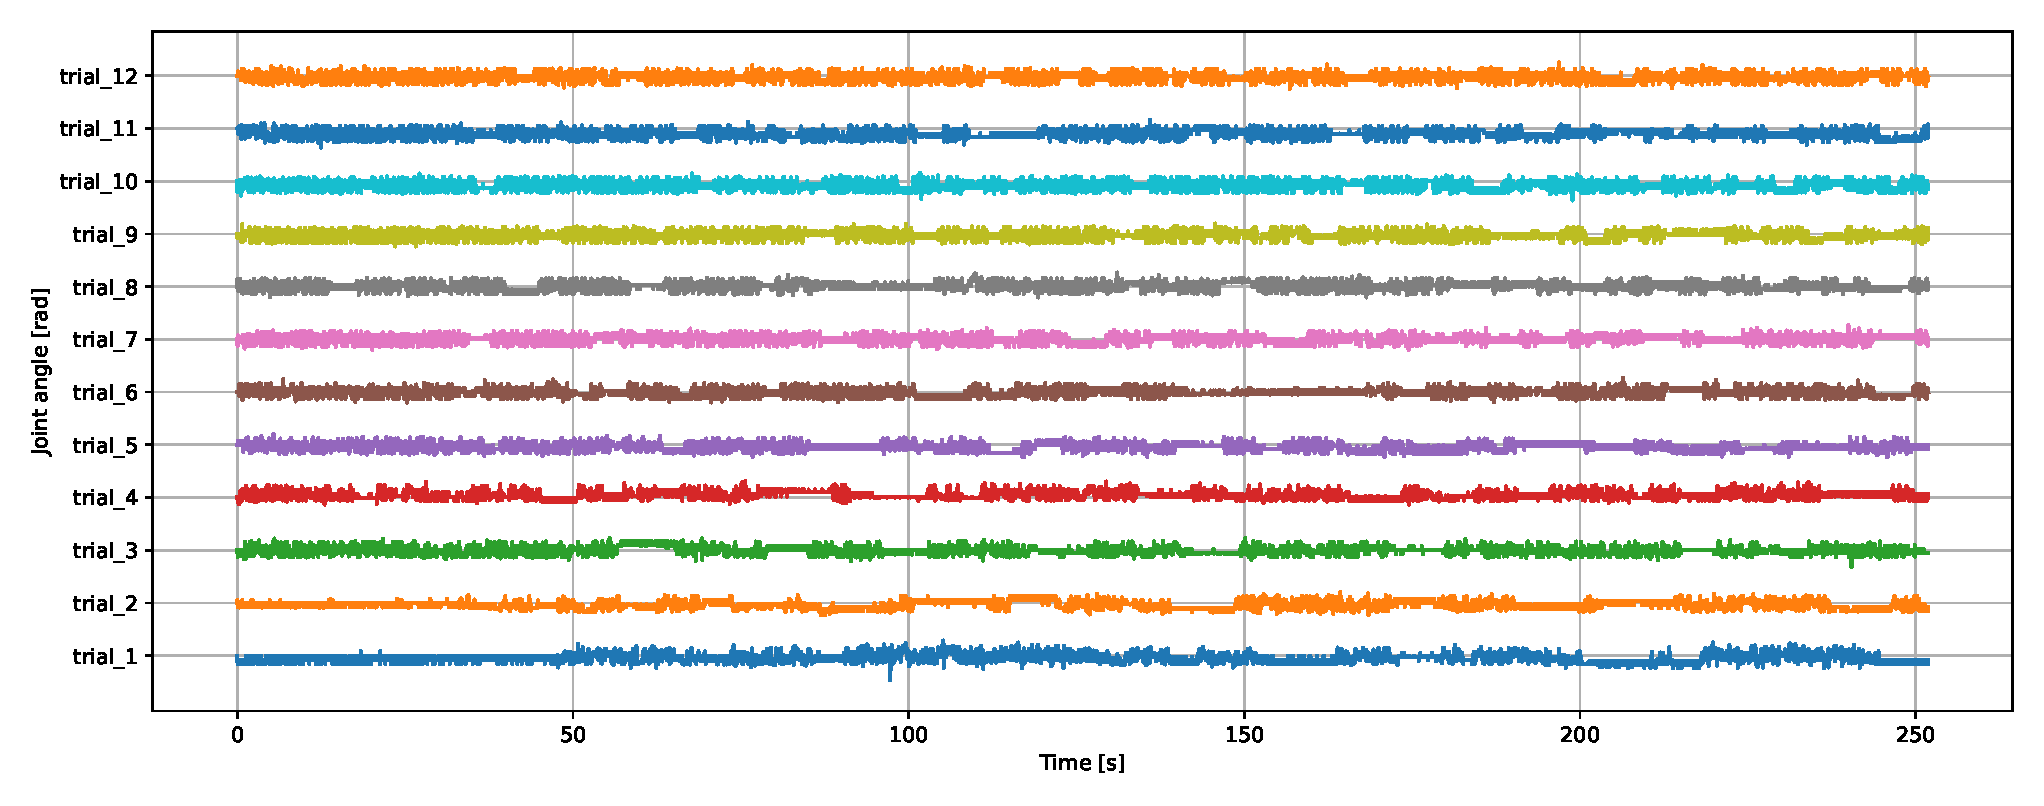
\includegraphics[width=\textwidth]{angle_angle_LH_leg_Coxa_yaw}
			\caption{left hind Coxa yaw angle}
			\label{fig::lh_coxa_yaw}
		\end{center}
	\end{subfigure}
	
	\begin{subfigure}[h]{0.6\textwidth}
		\begin{center}
			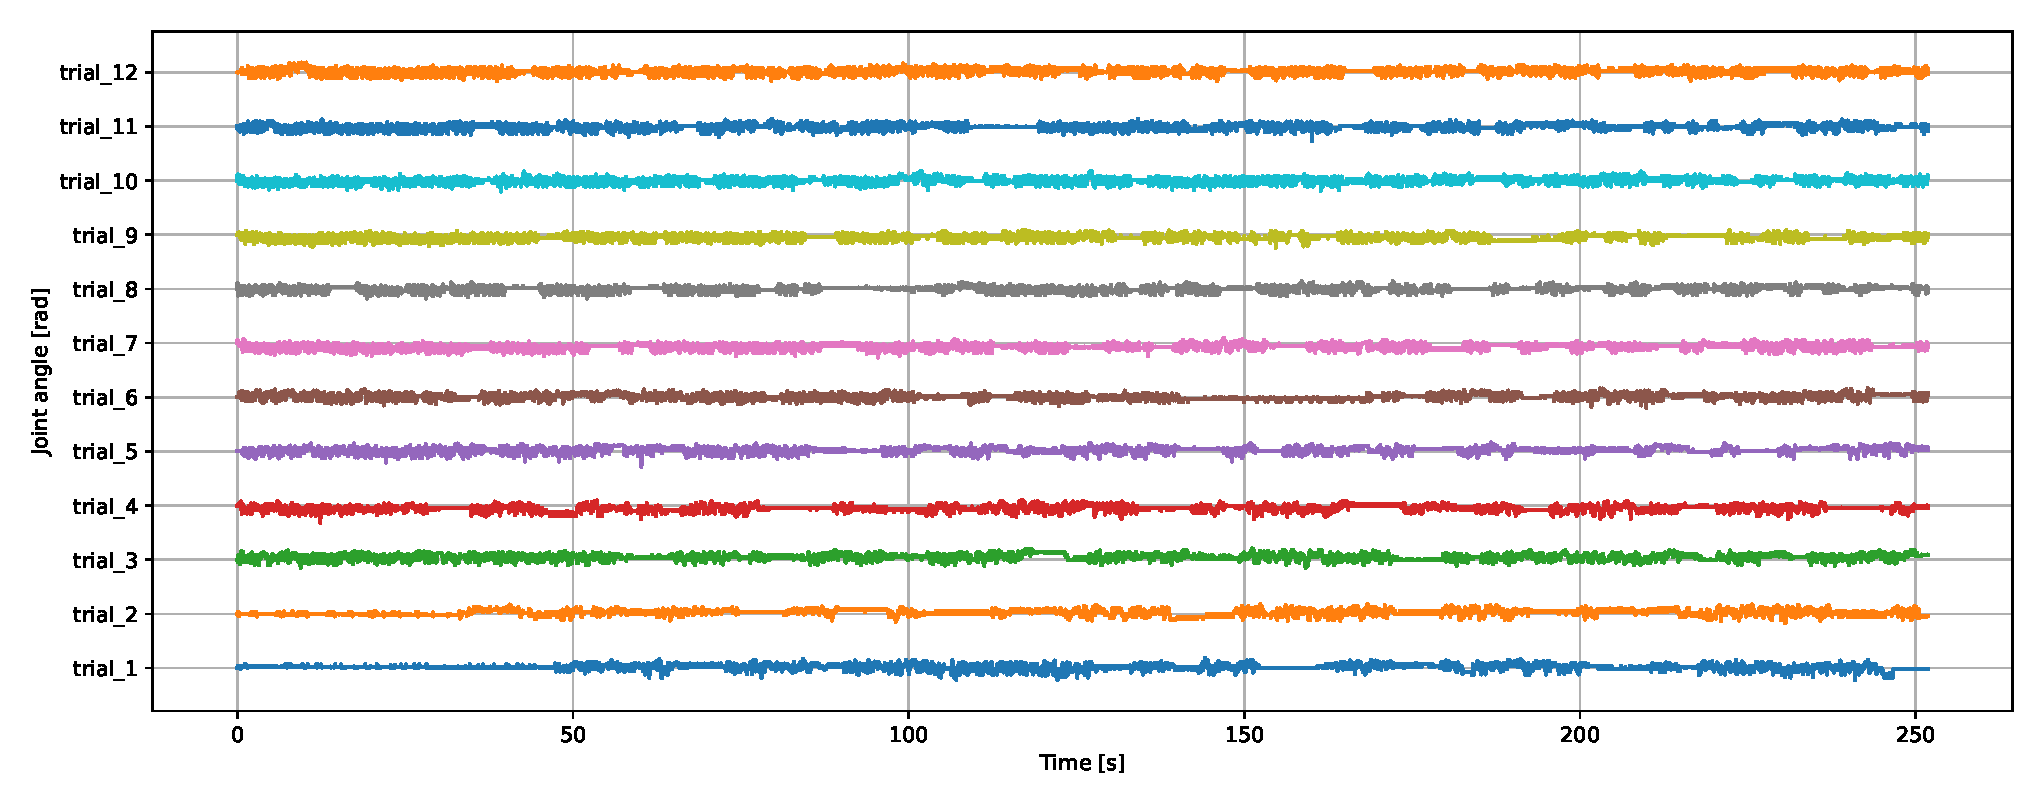
\includegraphics[width=\textwidth]{angle_angle_RF_leg_Coxa_yaw}
			\caption{right front Coxa yaw angle}
		\end{center}
	\end{subfigure}
	
	\begin{subfigure}[h]{0.6\textwidth}
		\begin{center}
			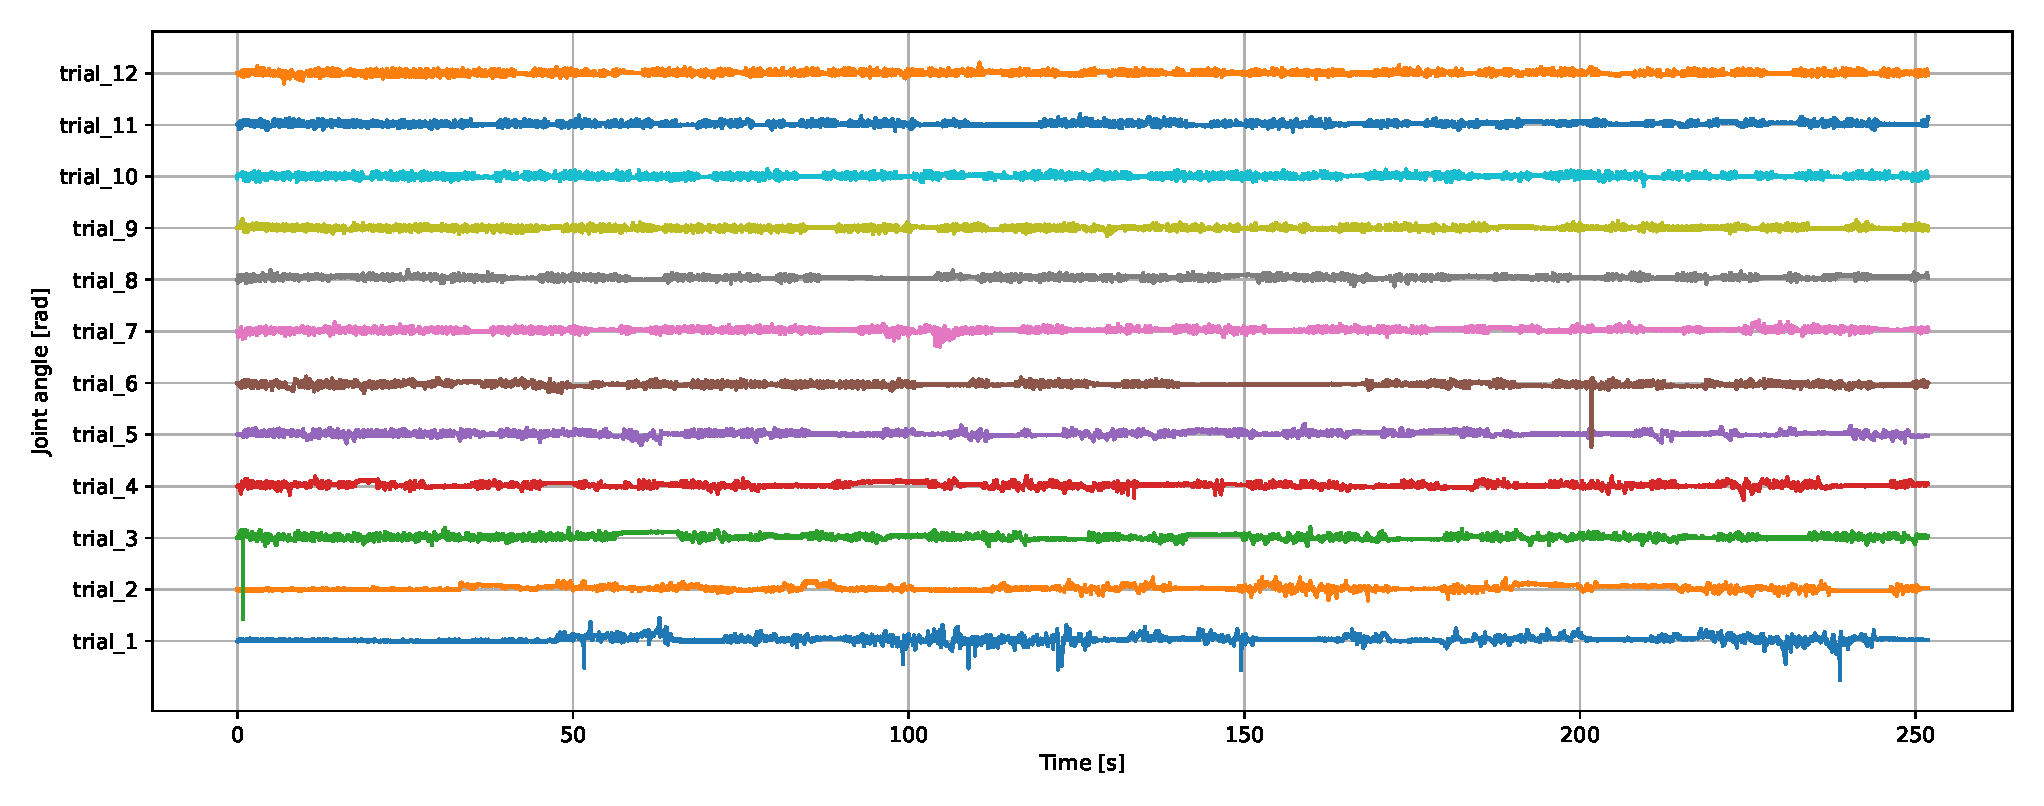
\includegraphics[width=\textwidth]{angle_angle_RH_leg_Coxa_roll}
			\caption{right hind Coxa roll angle}
		\end{center}
	\end{subfigure}
	\caption{A few joint angle signals as provided in the data set.}
	\label{fig::joint_angle}
\end{figure}

\begin{figure}[H]
	\begin{subfigure}[h]{0.6\textwidth}
		\begin{center}
			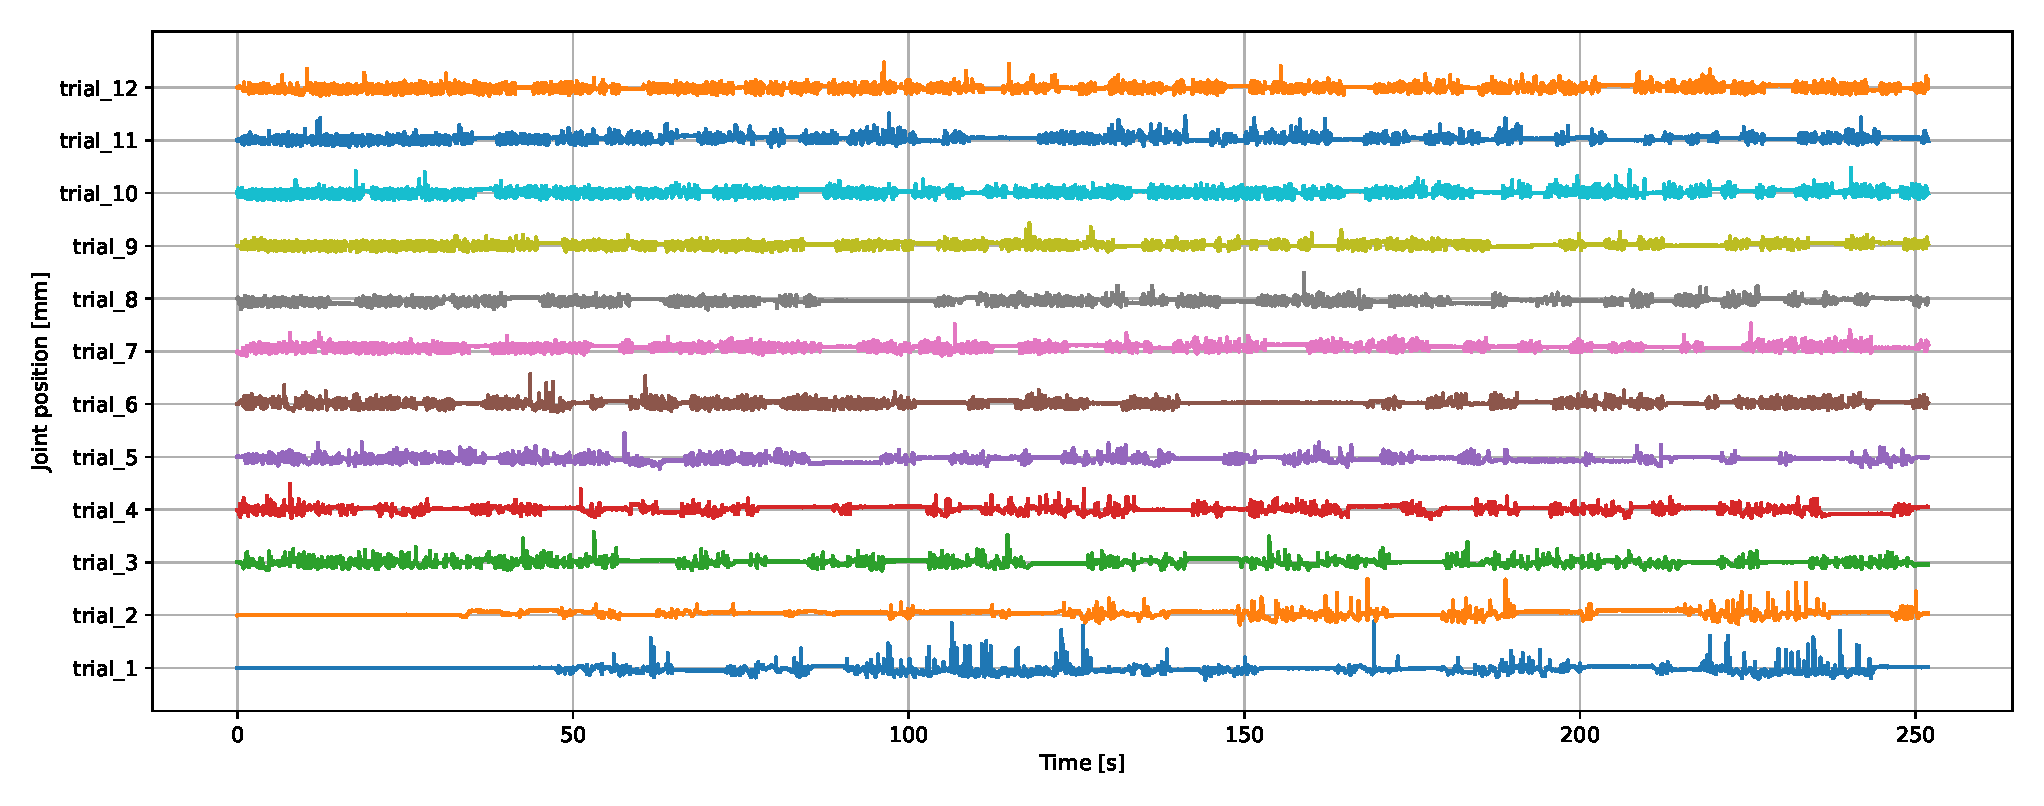
\includegraphics[width=\textwidth]{position_joint_LH_leg_Claw_z}
			\caption{left hind Claw $z$ position}
			\label{fig::lh_claw_z}
		\end{center}
	\end{subfigure}
	
	\begin{subfigure}[h]{0.6\textwidth}
		\begin{center}
			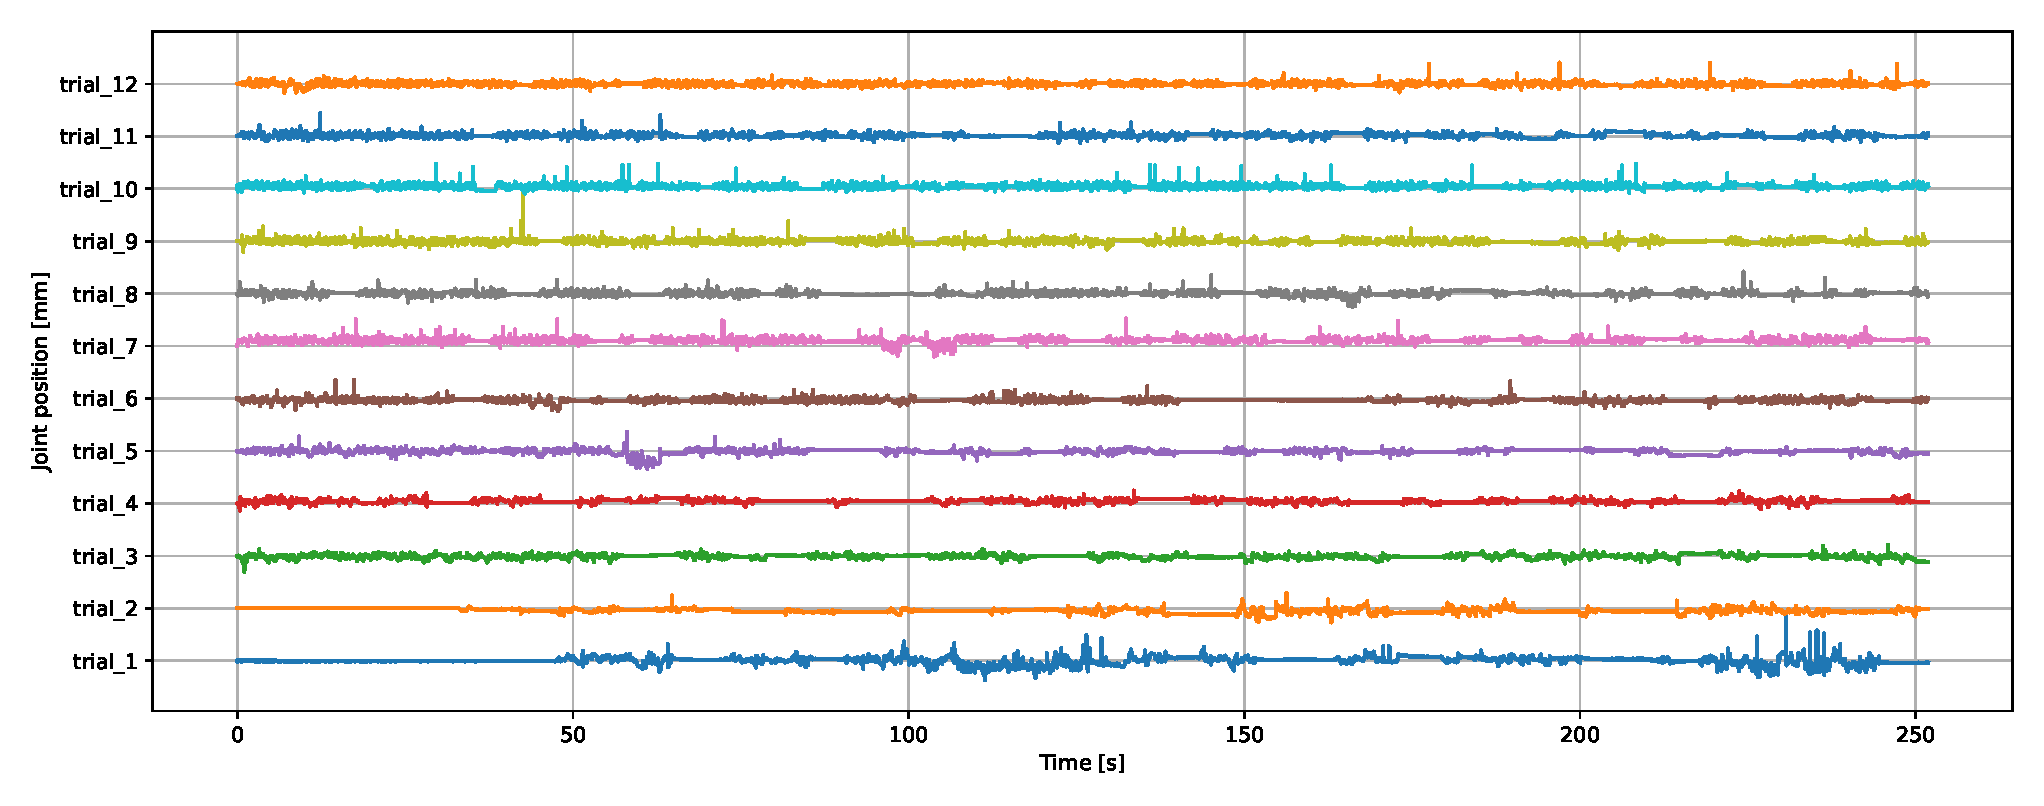
\includegraphics[width=\textwidth]{position_joint_LH_leg_Tarsus_y}
			\caption{left hind Tarsus $y$ position}
			\label{fig::lh_tarsus_y}
		\end{center}
	\end{subfigure}
	
	\begin{subfigure}[h]{0.6\textwidth}
		\begin{center}
			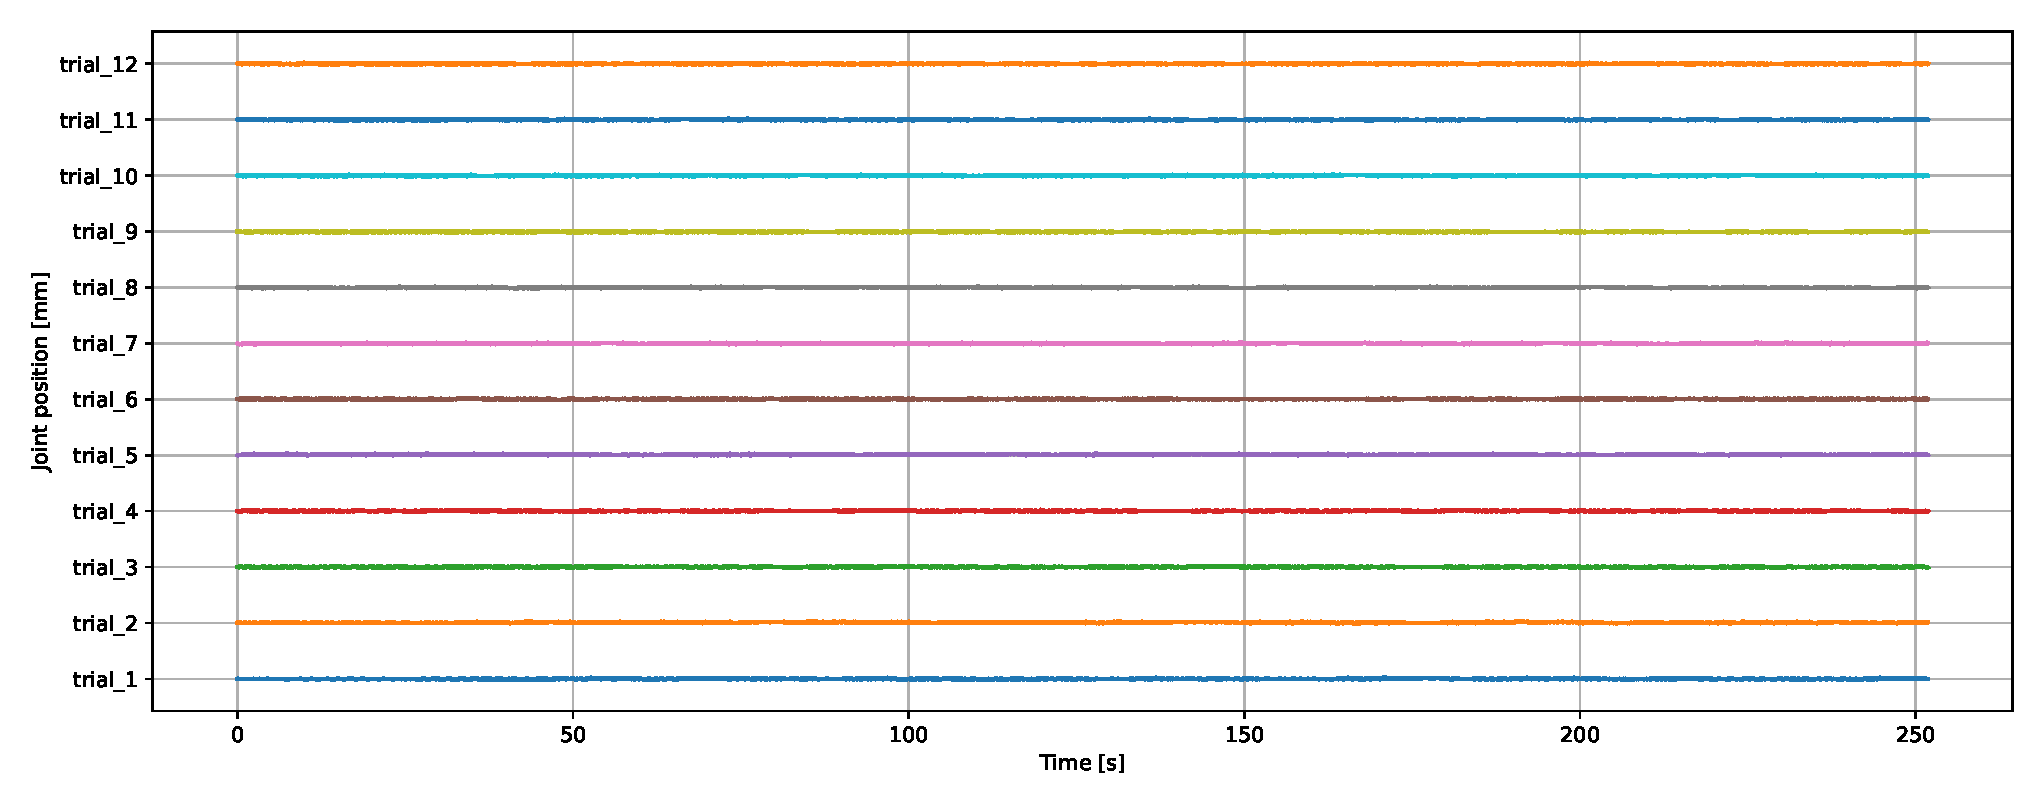
\includegraphics[width=\textwidth]{position_joint_RF_leg_Coxa_z}
			\caption{right front Coxa $z$ position}
			\label{fig::rf_coxa_z}
		\end{center}
	\end{subfigure}
	\caption{A few joint position signals as provided in the data set.}
	\label{fig::joint_position}
\end{figure}

We can see that some segments, within specifics degree of freedoms, are consistently immobile across the trials, like the right front Coxa $z$ position,~\ref{fig::rf_coxa_z}; while some are consistently mobile, like the left hind Coxa yaw angle (\ref{fig::lh_coxa_yaw}) or the left hind Tarsus $y$ position (\ref{fig::lh_tarsus_y}).

The signals do not display easily recognizable or repetitive patterns across the trials, which makes sense since they depend on the fly's behavior during the trial.

The joint angle data provides good behavioral characterization because they are a relative measure with respect to the fly's leg segments, and so will be really useful for the subsequent analysis.
The joint positions are also helpful but they give less insight, since similar behavior can results in different values, because of the absolute nature of the joint position signal with respect to the fly's leg segments.

\subsection{Neural data}

Neural data was recorded at \SI{16}{\hertz} using two-photon imaging, and was provided as 123 neural signal for all 12 trials.
Because two-photon imaging depends on relative change of fluorescence, the signals require to be normalized.
For that, a baseline was determined and subtracted.
Here it was computed as the minimum of a moving average of the signal over 10 frames for each neuron and each trial.
It makes sense to have independent baselines across neurons and trials, because the hypothesis is that the trials and neurons \textit{recordings} are independent.

\vspace{\baselineskip}

On Figure~\ref{fig::neural_before} below, we can observe a few examples of the neural signals:

\begin{figure}[H]
	\begin{subfigure}[h]{0.6\textwidth}
		\begin{center}
			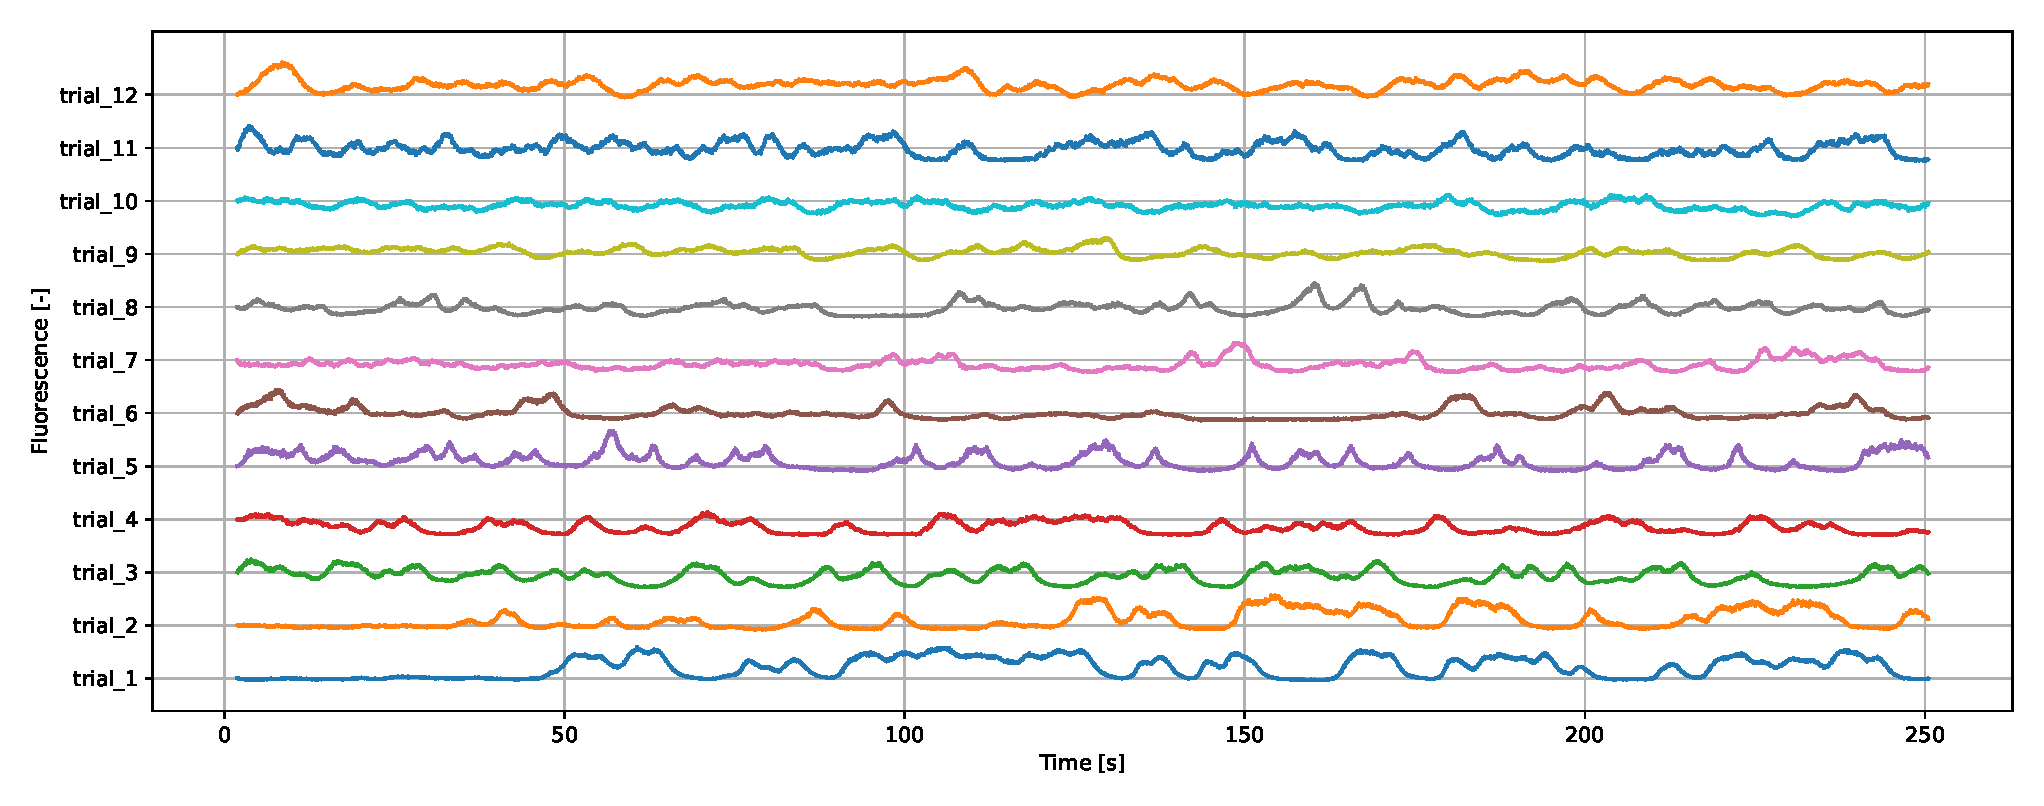
\includegraphics[width=\textwidth]{fluorescence2}
			\caption{neuron 2}
		\end{center}
	\end{subfigure}
	
	\begin{subfigure}[h]{0.6\textwidth}
		\begin{center}
			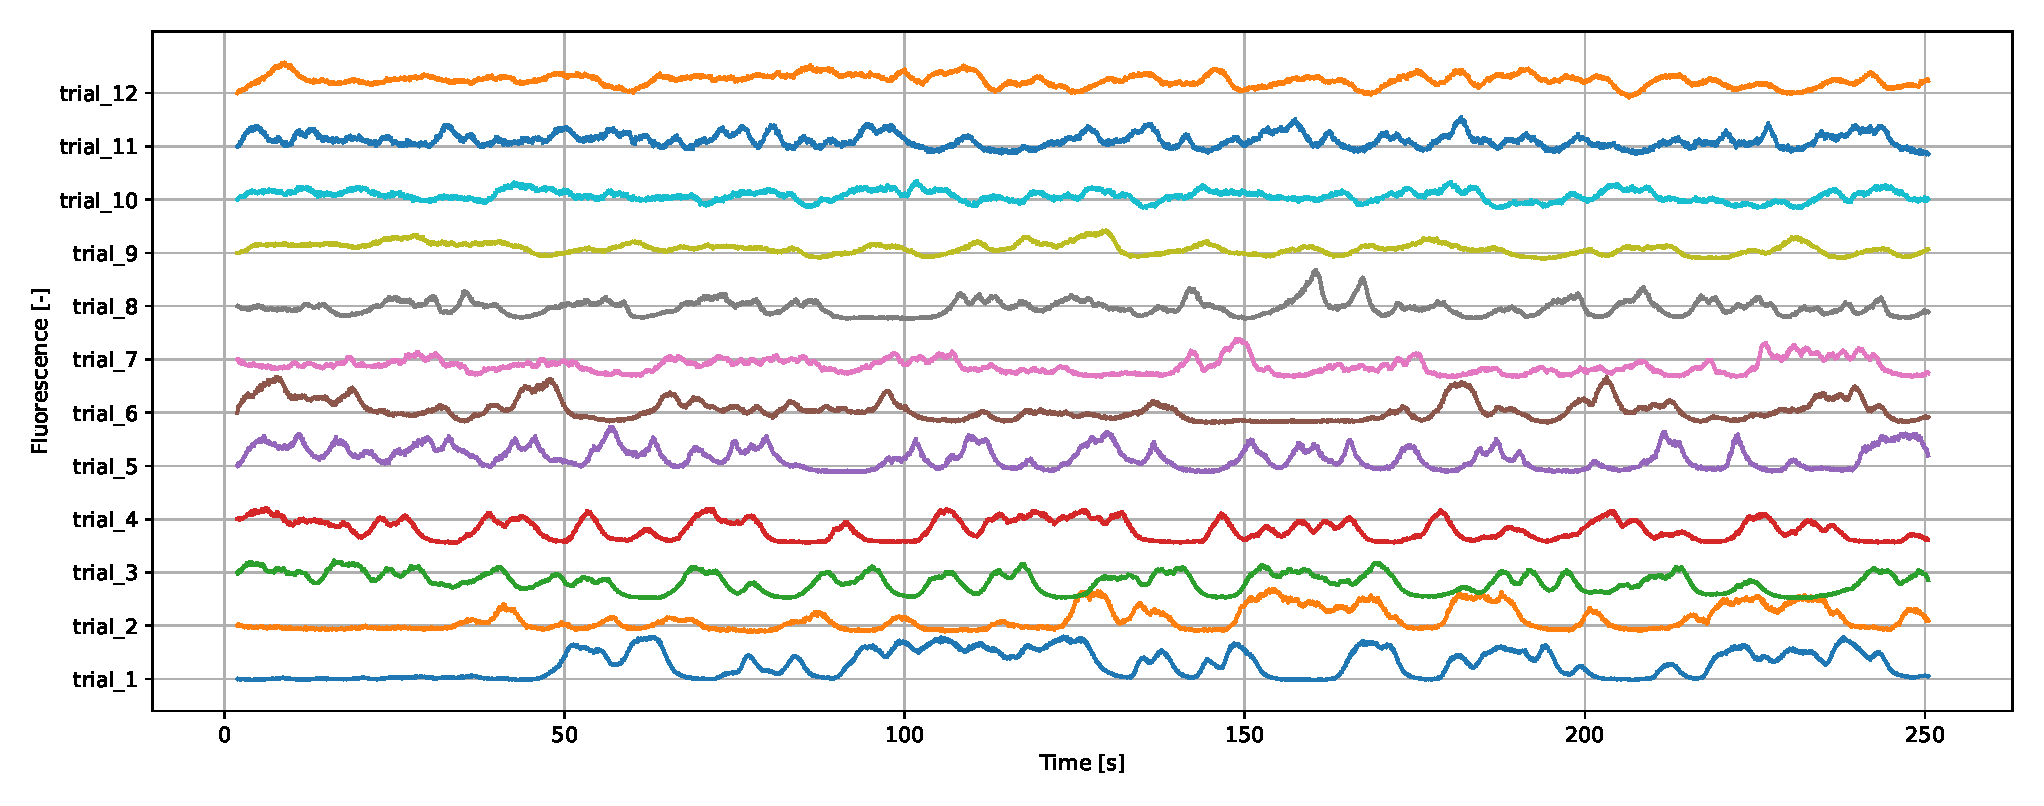
\includegraphics[width=\textwidth]{fluorescence7}
			\caption{neuron 7}
		\end{center}
	\end{subfigure}
	
	\begin{subfigure}[h]{0.6\textwidth}
		\begin{center}
			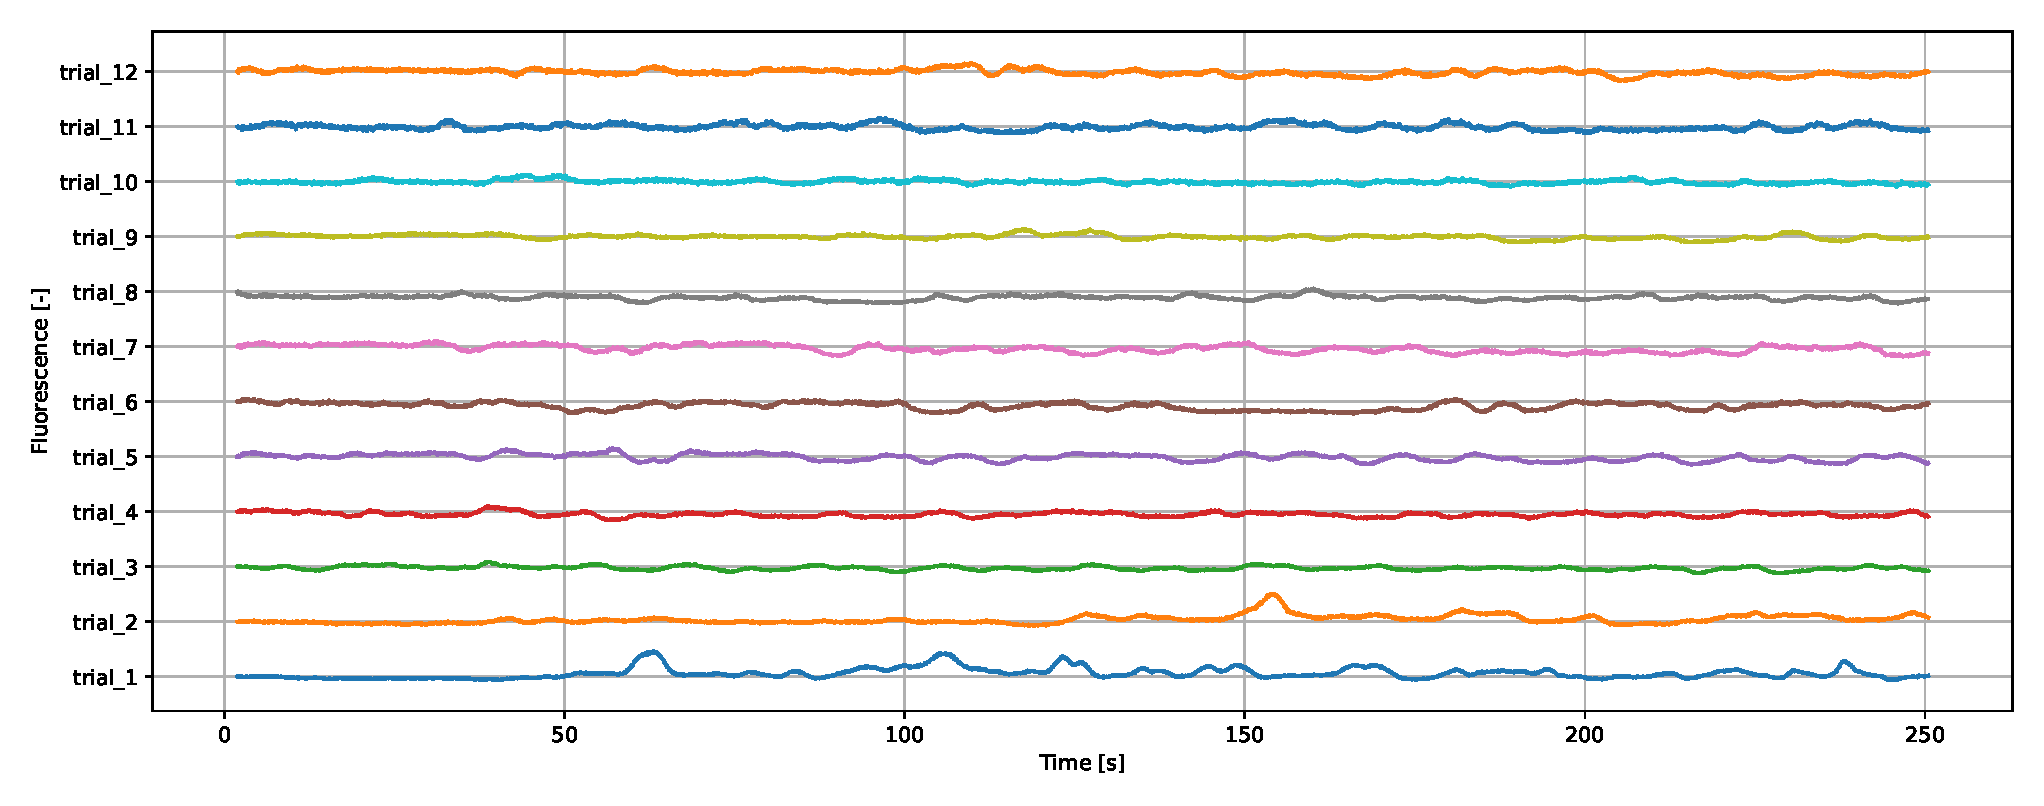
\includegraphics[width=\textwidth]{fluorescence42}
			\caption{neuron 42}
		\end{center}
	\end{subfigure}
	\caption{Neural signals after baseline subtraction (two-photon imaging produces data with an arbitrary unit).}
	\label{fig::neural_before}
\end{figure}

As can be seen on Figure~\ref{fig::neural_before}, the neural signals are quite noisy, and require low-pass filtering.
The noise is typical of in vivo recordings, and is mainly due to small voltage fluctuations in the neuron membrane as well as noise from the recording process. 

\begin{figure}[H]
	\begin{center}
		\includesvg[width=0.5\textwidth]{noise}
	\end{center}
	\caption{Window of neural fluorescence with different filters applied for noise reduction assessment.}
	\label{fig::neural_denoizing}
\end{figure}

On Figure~\ref{fig::neural_denoizing}, we can see that a Gaussian filter with $\sigma=6$ is appropriate to reduce the noise in a satisfactory manner.

\vspace{\baselineskip}

A few samples of the neural data after noise reduction are displayed on Figure~\ref{fig::neural_after} below:

\begin{figure}[H]
	\begin{subfigure}[h]{0.6\textwidth}
		\begin{center}
			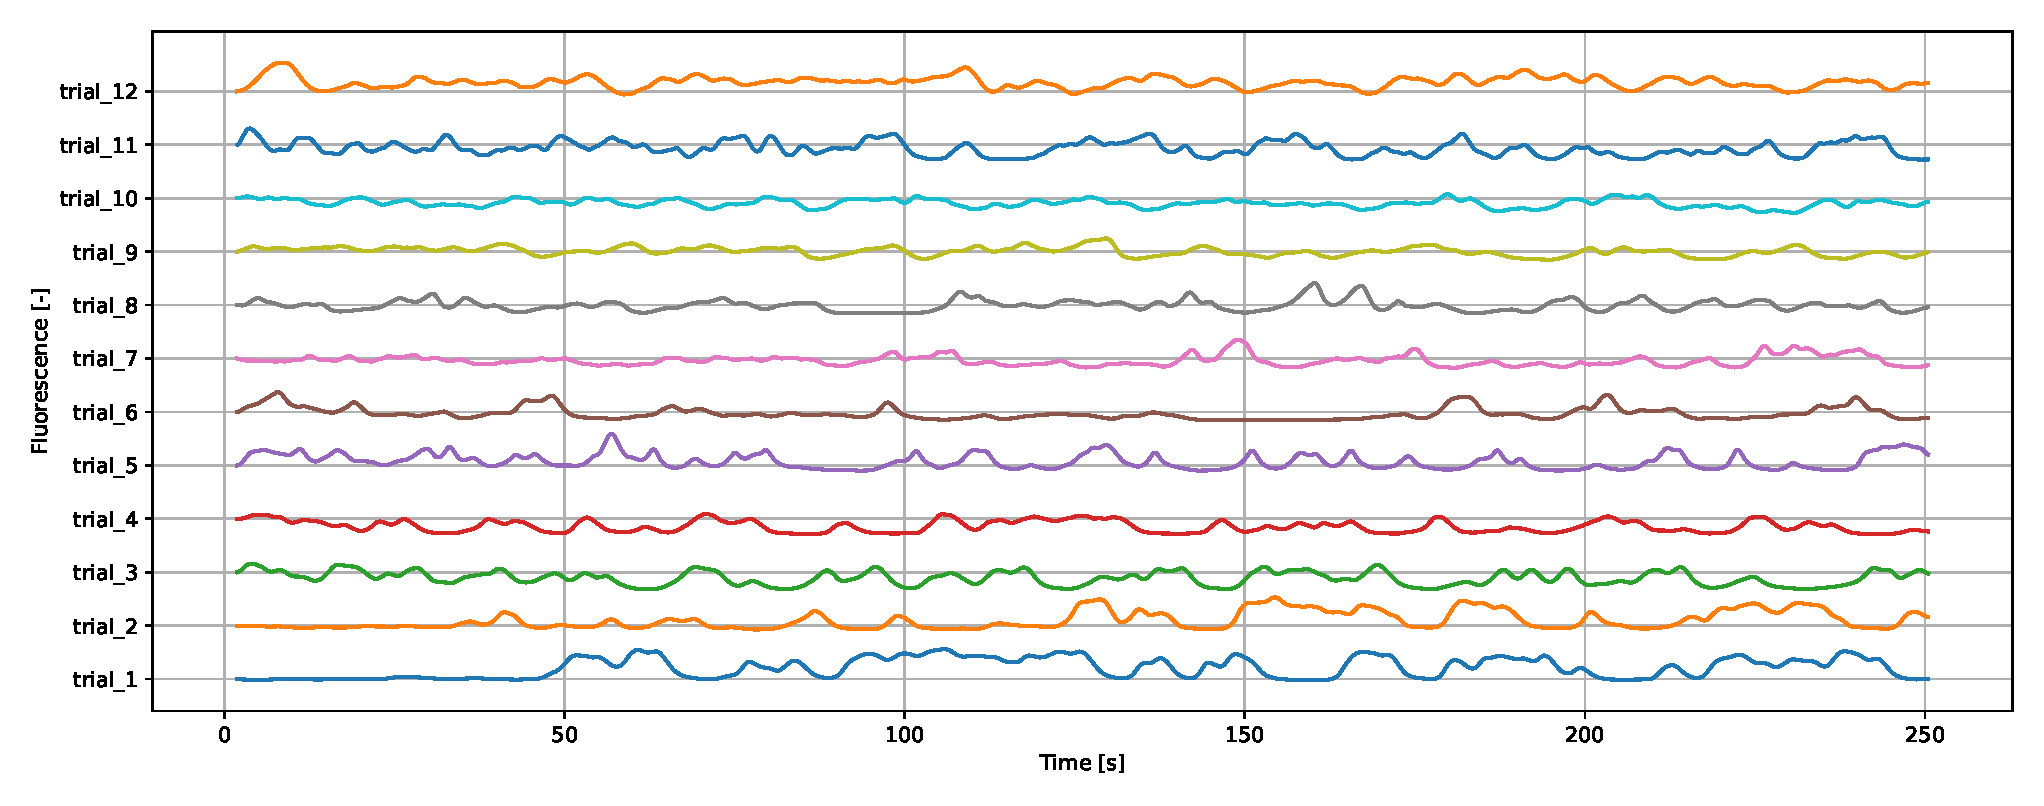
\includegraphics[width=\textwidth]{fluorescence_denoized2}
			\caption{neuron 2}
		\end{center}
	\end{subfigure}
	
	\begin{subfigure}[h]{0.6\textwidth}
		\begin{center}
			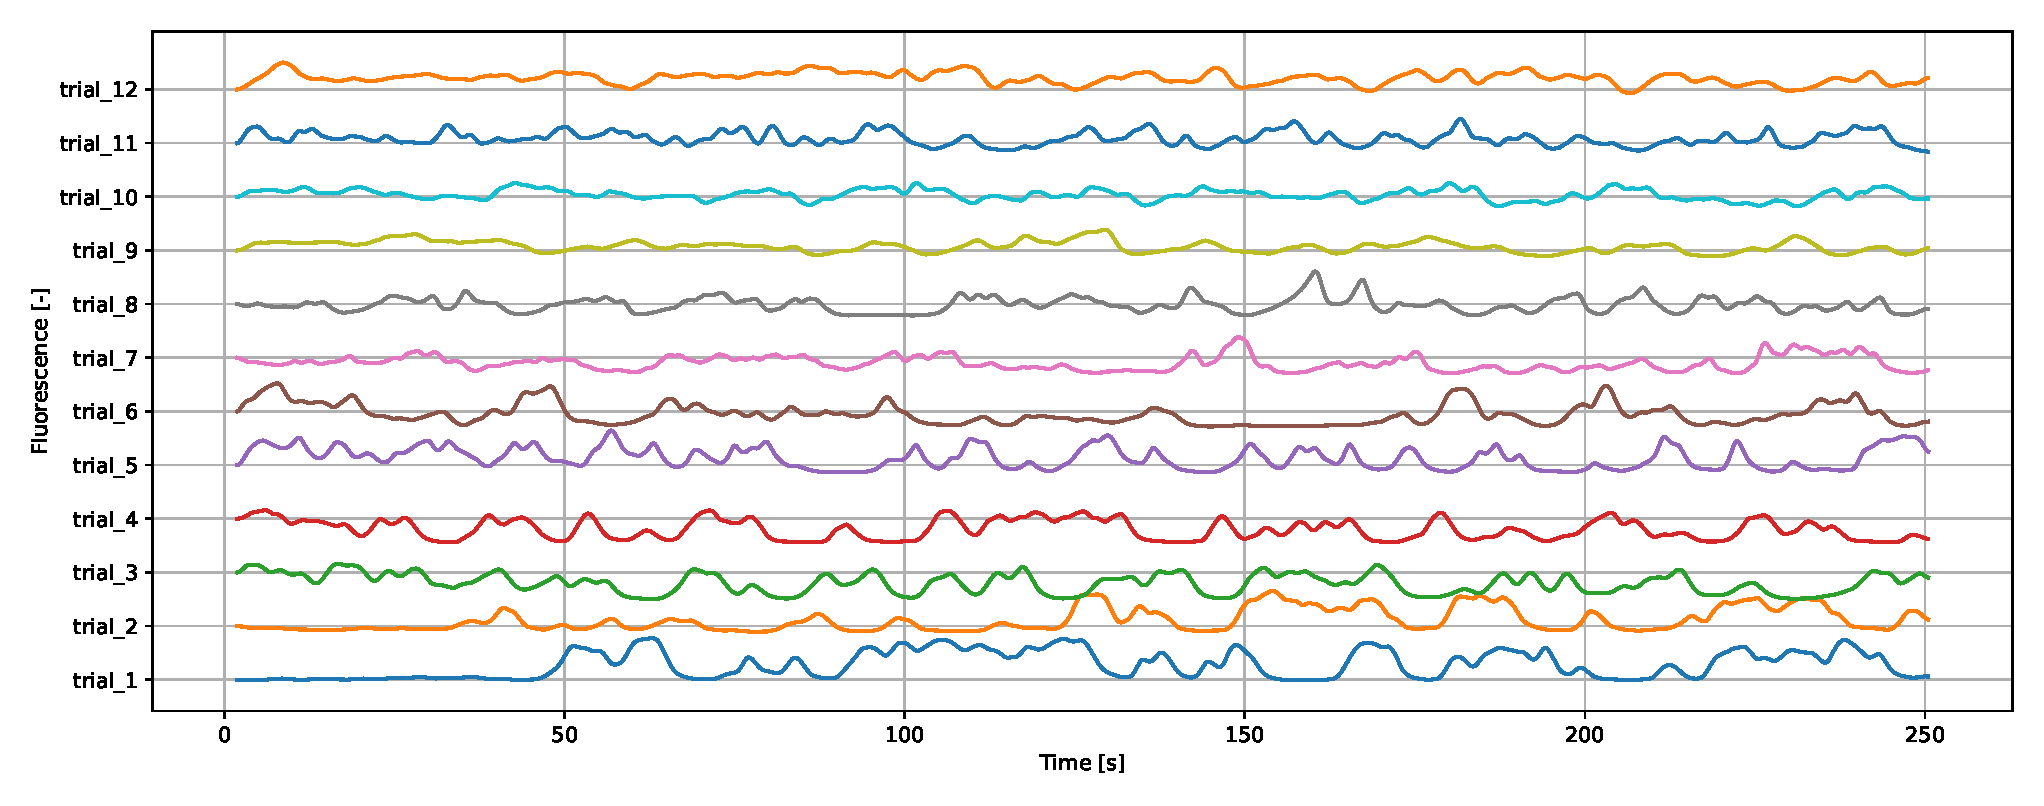
\includegraphics[width=\textwidth]{fluorescence_denoized7}
			\caption{neuron 7}
		\end{center}
	\end{subfigure}
	
	\begin{subfigure}[h]{0.6\textwidth}
		\begin{center}
			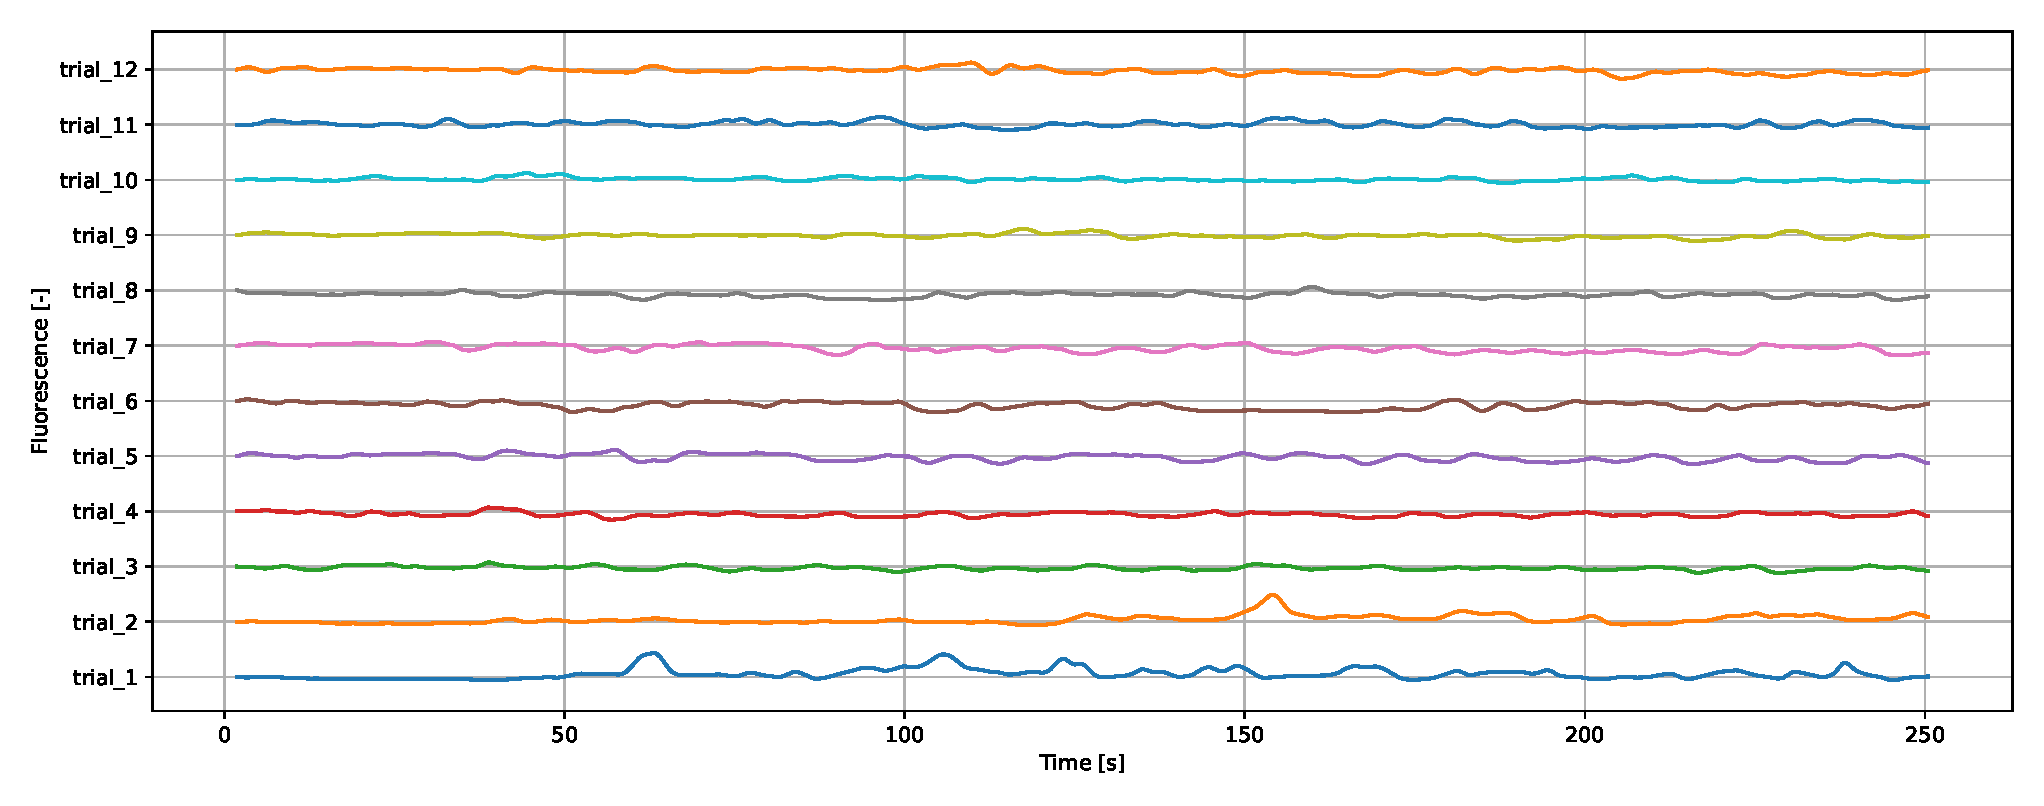
\includegraphics[width=\textwidth]{fluorescence_denoized42}
			\caption{neuron 42}
		\end{center}
	\end{subfigure}
	\caption{Neural signals after noise reduction (two-photon imaging produces data with an arbitrary unit).}
	\label{fig::neural_after}
\end{figure}

They are the same neurons as on Figure~\ref{fig::neural_before}, and when comparing both, it is visible that the noise reduction is satisfactory: most of the information is kept, while most of the noise is removed.

From these signals, the main observation is that some neurons are much more active than others, some trials displays more activity than other, and that the signals exhibit varied values.
This is consistent with the fact that the data is observational, and the flies are free to behave on the air-suspended spherical treadmill.

\vspace{\baselineskip}

After this preprocessing, the neural data is ready to be used.

\newpage
